\chapter {現状と実使用に向けて}\label{chap:todo}

\section {現状}\label{sub:genjo}

シンタックスエラー,型エラー,Unbound valueエラーが起きないという制約の元に,OCamlに慣れるために必要な基礎的な構文を備えた.
現在OCaml Blocklyでサポートしている構文は,以下の通りである.使用例を図\ref{fig:ocamlBlocks}に示す.
\begin{itemize}
  \item {\tt bool}型,{\tt int}型,{\tt float}型,{\tt string}型.
  \item 2つ組のみのタプル,リスト,ラムダ式,関数適用.
  \item 論理演算,数値演算,{\tt fst},{\tt snd}などのビルトイン関数.
  \item リストのパターンマッチを行う{\tt match}文.
  \item {\tt in}を持つ{\tt let},{\tt in}を持たない{\tt let},{\tt let rec}(どの{\tt let}もコンテキストメニューから変更可.).
  \item 1引数のみのコンストラクタ定義.
\end{itemize}

\begin{figure}[h]
 \centering
 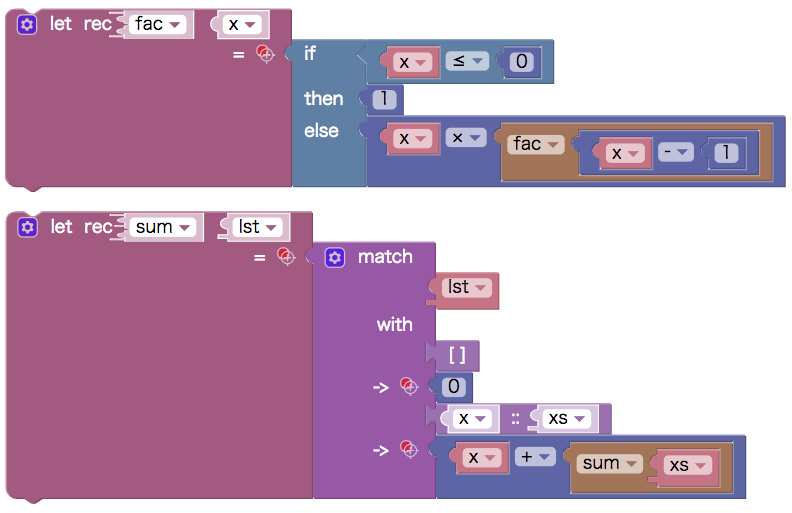
\includegraphics[keepaspectratio, scale=0.4]{img/ocamlBlocks1.png}
 \caption{OCaml Blockly でブロックを組み立てた例.
整数を受け取りその階乗を返す関数fac(上)と,整数の入ったリストを受け取りその合計を返す関数sum(下).\label{fig:ocamlBlocks}}
\end{figure}

\section {実使用に向けて}\label{sub:later}

第\ref{chap:senko}節にて掲げた最終的な目標は以下の2つであった.
\begin {enumerate}
  \item {\bf 「穴のないブロックを組み立てられた」ならば「コンパイルエラーの起きないプログラム」である}ことを保証する.
  \item 関数型言語初学者向けの授業で使えるクオリティにする.
\end {enumerate}

本論文では,この最終的な目標を見据えた上で,そのproof of conceptとなる目標を達成することができたと考えている.
今後は,現状のOCaml Blocklyの元にさらなる実装やテストを重ね,最終的な目標を達成していきたい.
そのために具体的に何を行なっていくか,どんな困難があるのか,といった点を本節で整理し,考察する.

\subsection*{コンパイルエラーの起きない制約}

本論文では,シンタックスエラー,型エラー,Unbound valueエラーを主要なコンパイルエラーとし,
この3つのエラーを起こすプログラムの組み立てを制限したユーザインタフェースを実装した.
%ブロックに穴があれば,生成されたプログラムは余裕でシンタックスエラーになってしまうため,ユーザへの警告が必要.
Unboundに関するエラーとしては,以降レコード型などの構文を追加していくに当たって,Unbound fieldなどといったエラーが起きうることが考えられるが,これはUnbound valueエラーを防いだ実装と同じような要領で回避することができる.

一方で,標準のOCamlで起きうるコンパイルエラーはシンタックスエラー,型エラー,Unboundエラーの3つだけではない.
例えば,「{\tt let rec f = f}」というプログラムは,2つ目のfの出現を指して,
「{\tt This kind of expression is not allowed as right-hand side of `let rec'}」というコンパイルエラーになるし,
「{\tt match ... with x ::\ x -> ...}」といったプログラムは
2つ目のパターン変数xを指して「{\tt Variable x is bound several times in this matching}」というエラーになってコンパイルが失敗する.

これらのコンパイルエラーを起こすプログラムをブロック上で組み立てられないよう,
OCaml Blockly上でのエラーのチェックを拡張していく必要があるが,その方法は主に2つある.

1つは,各種エラーを逐一対応していき,アドホックな変更を重ねることである.
この方法は,数種類のエラーだけを対応するならば,手っ取り早く確実であるが,
全てのコンパイルエラーを防ぐためには,スケールしない方法と言える.
OCaml BlocklyはOCamlという膨大な言語処理のとても局所的な部分をJavaScript上で「再現」しているため,
OCamlにおけるコンパイルエラーと一貫性を保つのは困難である.

2つ目の方法は,compiler-libsを利用して実際にコンパイルを行い,そのコンパイルエラーを流用することである.
抽象構文木にブロック上の穴を表現するための構文を追加し,ブロックを抽象構文木に落せるようにして,コンパイルを行う.
コンパイルエラーが起きたら,そのエラーを返す.このプログラムをjs\_of\_ocamlでビルドすれば,ブラウザ上で用いることができる.
この方法は,OCamlにおけるコンパイルエラーとの一貫性を確実に実現できるが,
お砂場を含むワークスペースにある全ブロックとテキストによるOCamlコードの対応関係を的確に保たなければいけない.

\subsection*{さらなる構文}

新しい構文をただ単にブロックに追加するのは容易であるが,
「不正なプログラムを組み立てられない」というOCaml Blocklyの制約を維持しながらの構文の追加は自明でない.

例えば,ユーザの動作によってあらゆる箇所のブロックが動的に変更された場合にどう対応するかという仕様を考えなければならない.
コンストラクタを定義するブロックが変更されたとき,コンストラクタ呼び出しはどう変わるべきか,
その引数に自由変数が入っていたらどうなるべきか.%let recのブロックを組み立て終えたところで,ユーザがrecフラグを突然削除したら再帰呼び出しブロックはどうするべきか.
また,let文の引数宣言を削除したときに,引数を参照していた変数ブロックはどうなるべきか.

他にも,ブロックのユーザインタフェースとどう合わせるのかを考える必要がある.
例えば,変数を持つパターンブロックがmatchブロックに接続されたときに,変数宣言としてどう見せるべきなのか,
可変長の要素を持つブロックであれば,それをどうユーザに操作させるのが適切か,などと言った問題がある.
これらの問題を考えると,構文と構文が表す概念をOCaml Blocklyの世界に載せるには時間が必要である.

本論文では,ユニットテストで様々な組み合わせのプログラムを機能させ続けることに注意を払つつ,
OCaml Blocklyでの各構文の仕様を決め,種類を少しずつ足していった.
基礎的な構文が実現できた今,OCamlの授業で使用するために,次に追加する必要のある構文を以下にまとめた.

\begin{itemize}
  \item 柔軟なコンストラクタ定義,レコード型.
  \item 可変長のタプル.
  \item 豊富なマッチパターン.
  \item Listモジュール関数.
\end{itemize}

OCamlで様々なデータセットを扱うために,コンストラクタ,レコード型といった柔軟なユーザ定義のデータ型を実現したい.
また,現状ではタプルは2つ組のみしかサポートしていないが,可変長のタプルを追加する.
次は,関数型言語の重要な特徴の1つといえるmatch文のパターンを豊富にすることである.
現在は{\tt x ::\ xs},{\tt []}といった2つのパターンのみが使えるが,これを拡張し,
例えば{\tt (a, b)}や,再帰的なパターン{\tt (a, b) ::\ xs}を表現できるようにする.
最後は,Listモジュールのサポートである.

これ以上の構文は,実際に授業のカリキュラムに合わせてテストをした際に,
必要な構文があれば随時サポートしていく指針だ.
%もっと最終目標言うべき?

\subsection*{ユーザビリティの点から}

使いやすさ,理解しやすさの達成するためには,まず第一に初学者にテストしてもらいフィードバックをもらう必要がある.
フィードバックに基づき,OCaml Blocklyのユーザインタフェースに関わる部分を改善していく.

一方で,著者が実際に使用してみたとき,実使用に向けて,使い勝手の点から設計や実装が必要だと考える点は以下の2つである.%4つ?
\begin{itemize}
 \item OCamlの構文に合わせたブロックのユーザインタフェースの改造.
 \item 型を視覚的に表示することによる限界.
% \item Undo機能の実装.
\end{itemize}

まず始めに,OCamlの構文に沿ってブロックのユーザインタフェースを改造する必要がある.
現在ブロックそのものに関するユーザインタフェースはほとんど変えていない.
もともとBlocklyはビジュアルプログラミング言語環境を構築するためのライブラリであり,
1つの言語に特化した設計にはなっていないが,
どちらかというと命令型言語との方が相性が良く,関数型言語のような文より式が主な言語をそのまま載せると,
元のBlocklyにあった直感的なユーザ体験を損ないがちである.図\ref{fig:ocamlBlocks}では,
letブロックの左側の余白部分が大きいせいで,代入や出力の関係が捉えにくくなってしまっている.
初学者にとってOCamlの言語仕様をより直感的に理解してもうらためには,
OCamlの言語仕様に特化したビジュアルのデザインが不可欠である.

また,型を視覚的に表示することには限界がある.
型によってコネクタの形を変える\cite{Typed-Blockly}のアイデアは,
プリミティブ型に関してはとても有効である.
一方で,Function型などといったパラメタ付型を形で表すことは,型が入れ子になって複雑になるほど,逆に理解をさせにくくしてしまう.
入れ子になる型は視覚的に表示することをやめて,ホバー時にツールチップの形で出力する,などといった策を取る必要がある.

%最後の1つは,OCaml Blocklyでのundoの実装である.%この段落の説明が微妙
%ユーザが誤ってブロックを削除してしまったとき,undo機能があればストレス無く元の作業に戻ることができる.
%本来のBlocklyではundoやredoが実装されているが,
%作業空間がメインワークスペースのみであるために,undo機能を実現するためのユーザの動作の記録はメインワークスペースのみに行われている.
%対して,OCaml Blocklyにはお砂場という別の作業空間があるため,動作の保持をグローバルに行うよう拡張する必要がある.

%是非そういうところに注目してみてほしい!!

% blockly/blockly/demos/interpreter/step-execution.html


